\providecommand{\main}{..}
\documentclass[\main/main.tex]{subfiles}
\begin{document}

\chapter{Introduction}
\section{Why is the Zipf interesting?}
The Zipf law is an empirical law that refers to the fact that in nature, many data can be approximated by a Zipfian distribution, for example texts, some images\footnote{https://www.dcs.warwick.ac.uk/bmvc2007/proceedings/CD-ROM/papers/paper-288.pdf}, even sounds in spoken languages\footnote{https://journals.plos.org/plosone/article?id=10.1371/journal.pone.0033993}. It is therefore of interest to identify ways to exploit this relatively simple way to convert documents into representative vectors in problems such as classifications.

\begin{figure}
  \begin{subfigure}{0.32\textwidth}
    
\includegraphics[width=\textwidth]{introduction/books}
    \caption{Books follow a zipf distribution}
  \end{subfigure}
  \begin{subfigure}{0.32\textwidth}
    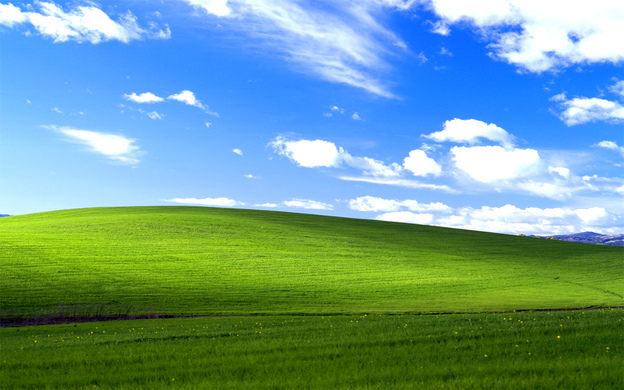
\includegraphics[width=\textwidth]{introduction/image}
    \caption{Image formats such as jpeg follows a zipf distribution}
  \end{subfigure}
  \begin{subfigure}{0.32\textwidth}
    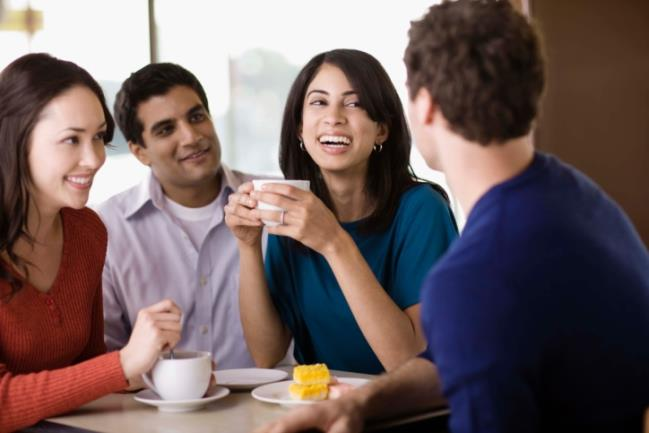
\includegraphics[width=\textwidth]{introduction/people}
    \caption{Sounds in spoken language follow a zipf distribution}
  \end{subfigure}
  \caption{Examples of things in nature that follows the zipf distribution}
\end{figure}

\section{What is attempted in this project?}
In this project was attempted to classify textual documents using the bag of words model, ignoring any semantic structure, to their class using a general clustering approach with algorithms such as KMeans and CURE. No heuristics relative to the nature of the texts was used.

\end{document}